\iffalse
\let\negmedspace\undefined
\let\negthickspace\undefined
\documentclass[journal,12pt,twocolumn]{IEEEtran}
\usepackage{cite}
\usepackage{amsmath,amssymb,amsfonts,amsthm}
\usepackage{algorithmic}
\usepackage{graphicx}
\usepackage{textcomp}
\usepackage{xcolor}
\usepackage{txfonts}
\usepackage{listings}
\usepackage{enumitem}
\usepackage{mathtools}
\usepackage{gensymb}
\usepackage{comment}
\usepackage[breaklinks=true]{hyperref}
\usepackage{tkz-euclide}
\usepackage{listings}
\usepackage{gvv}
\def\inputGnumericTable{}
\usepackage[latin1]{inputenc}
\usepackage{color}
\usepackage{array}
\usepackage{longtable}
\usepackage{calc}
\usepackage{multirow}
\usepackage{hhline}
\usepackage{ifthen}
\usepackage{lscape}

\newtheorem{theorem}{Theorem}[section]
\newtheorem{problem}{Problem}
\newtheorem{proposition}{Proposition}[section]
\newtheorem{lemma}{Lemma}[section]
\newtheorem{corollary}[theorem]{Corollary}
\newtheorem{example}{Example}[section]
\newtheorem{definition}[problem]{Definition}
\newcommand{\BEQA}{\begin{eqnarray}}
\newcommand{\EEQA}{\end{eqnarray}}
\newcommand{\define}{\stackrel{\triangle}{=}}
\theoremstyle{remark}
\newtheorem{rem}{Remark}
\begin{document}

\bibliographystyle{IEEEtran}
\vspace{3cm}

\title{NCERT Discrete - 10.5.2.19}
\author{EE23BTECH11007 - Aneesh Kadiyala$^{*}$% <-this % stops a space
}
\maketitle
\newpage
\bigskip

\renewcommand{\thefigure}{\theenumi}
\renewcommand{\thetable}{\theenumi}
\vspace{3cm}
\textbf{Question 10.5.2.19:} Subba Rao started work in 1995 at an annual salary of Rs. 5000 and received an increment of Rs. 200 each year. In which year did his income reach Rs. 7000?

\solution
\fi
\begin{table}[h!]
    \centering
    \begin{tabular}{ | c | c | c | }
        \hline
        Parameter & Value & Description \\
        \hline
        $x(0)$ & 5000 & Initial Income \\
        \hline
        $d$ & 200 & Annual Increment (Common Difference) \\
        \hline
        $x(n)$ & $(x(0) + nd)u(n)$ & $n^{th}$ term of the AP \\
        \hline
    \end{tabular}
    \caption{Input Parameters}
    \label{tab:math_10_5_2_19}
\end{table}
From the values given in \tabref{tab:math_10_5_2_19}:
\begin{align}
7000 &= 5000 + 200n \\
\implies 2000 &= 200n \\
\therefore n &= 10
\end{align}
\begin{figure}[h!]
    \centering
    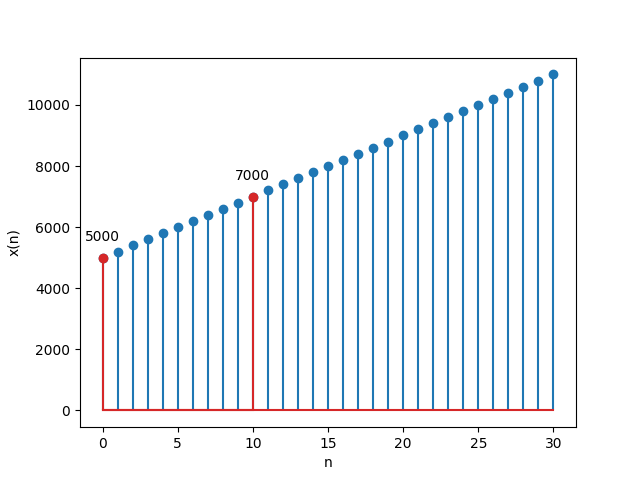
\includegraphics[width=\columnwidth]{ncert-maths/10/5/2/19/figs/10_5_2_19.png}
    \caption{Plot of $x(n)$ vs $n$. See \tabref{tab:math_10_5_2_19} for details.}
    \label{fig:math_10_5_2_19}
\end{figure}
Let Z-transform of $x(n)$ be $X(z)$.
\begin{align}
X(z) &= \frac{x(0)}{1 - z^{-1}} + \frac{dz^{-1}}{(1 - z^{-1})^2} \quad |z| > 1
\end{align}
Using the values from \tabref{tab:math_10_5_2_19}:
\begin{align}
X(z) &= \frac{5000}{1 - z^{-1}} + \frac{200z^{-1}}{(1 - z^{-1})^2} \quad |z| > 1
\end{align}
%\end{document}
